% !TeX root = bmvc_c3vd_benchmark_draft.tex
% !TeX program = pdflatex
\documentclass{bmvc2k}
\bmvcreviewcopy{1770}

\title{C3VDReg: Benchmarking Local Colonoscopic Registration for Anatomy-Aware Localization}

\addauthor{Anonymous BMVC Submission}{}{1}
\addinstitution{Anonymous Institution}

\runninghead{Anonymous BMVC Submission}{C3VDReg}

\def\eg{\emph{e.g}\bmvaOneDot}
\def\Eg{\emph{E.g}\bmvaOneDot}
\def\etal{\emph{et al}\bmvaOneDot}
\newcommand{\figpanel}[2]{\parbox[t]{#1}{\centering\normalsize #2}}
\newcommand{\figpanelleft}[2]{\parbox[t]{#1}{\raggedright\normalsize #2}}
\newcommand{\best}[1]{\textbf{#1}}
\newcommand{\second}[1]{\underline{#1}}
\emergencystretch=2em

\graphicspath{{images/}}

\begin{document}

\maketitle

\begin{abstract}
Clinically useful colonoscopic guidance requires the live endoscopic view to be localized on a stable 3D reference at any point in a procedure, enabling anatomy-aware overlays rather than only procedure-level or frame-level recognition. Such localization could support coverage assessment, revisited-region awareness, and, in the longer term, augmented guidance by linking intraoperative video with preoperative CT-derived anatomy. Yet rigid point cloud registration in the colon differs fundamentally from standard indoor or outdoor benchmarks: the surface is locally homogeneous, haustral folds are repetitive, observations are highly partial, and reconstructed depth is noisy and incomplete. We present C3VDReg, a dataset and benchmark derived from released Colonoscopy 3D Video Dataset (C3VD) camera poses, depth maps, and CT meshes. For each frame, C3VDReg generates a source point cloud by depth map reprojection and a target point cloud by raycasting the CT mesh from the matched camera pose. The benchmark contains 10,015 viewpoint-matched partial-to-partial point-cloud pairs, including 2,088 held out test pairs, and evaluates public baselines under a shared contract: 8,192 points per cloud, source-only perturbations, a fixed source-to-target pose convention, and common pose metrics. Across representative classical and learning-based methods, performance remains low. The strongest baseline, GeoTransformer, reaches only 17.43\% Registration Recall at 5deg/5mm and 35.63\% at 10deg/10mm. Ground-truth overlap is high (74.3--93.1\%), yet recall remains low and nonmonotonic with overlap, indicating that the main bottleneck is translation ambiguity in repetitive tubular anatomy rather than missing shared surface alone. C3VDReg provides a reproducible benchmark for measuring progress on this intermediate step toward local-to-global colonoscopic localization.
\end{abstract}

\section{Introduction}
\label{sec:intro}

Colonoscopy is central to colorectal cancer detection and surveillance, yet the moving endoscope observes only a small local patch of the mucosal surface at any instant~\cite{ma2021rnnslam,yao2021motion}. For deployment, clinicians need the current observation to be localized on patient anatomy throughout the procedure so that an overlay can be tied to the correct anatomical region rather than only to a recognized video frame. Linking the live view to a stable 3D anatomical reference could support anatomy-aware navigation, coverage assessment, revisited-region awareness, and lesion site contextualization in a common coordinate system~\cite{bobrow2023colonoscopy,ma2021rnnslam,yao2021motion,nayor2017endoscopic}. When CT-derived colon geometry is available, this objective can be viewed as registering intraoperative endoscopic observations to preoperative anatomy, an important step toward augmented colonoscopic guidance.

However, this registration problem is not well captured by standard point cloud benchmarks. Classical pipelines such as ICP and feature-based matching, as well as learning-based methods such as PointNetLK, DCP, RegTR, and GeoTransformer, are predominantly studied on CAD objects, indoor RGB-D scenes, or outdoor LiDAR data~\cite{pomerleau2015review,huang2021comprehensive}. The colon differs fundamentally from these settings. Its surface is locally homogeneous, haustral folds repeat over long extents, each endoscopic frame provides only a highly partial observation, and reconstructed depth is noisy and incomplete. These properties make reliable keypoint detection difficult, create feature descriptor degeneracy and matching ambiguity, and can yield severe translation uncertainty even when local residuals look plausible.

Existing colonoscopy datasets provide important assets for depth estimation, pose estimation, reconstruction, and procedure-level perception, but they do not define a fixed benchmark for rigid point cloud registration between video-derived observations and CT-derived anatomy~\cite{bobrow2023colonoscopy,lena2026realsyncol,rau2024simcol3d,biffi2024realcolon,ju2024segcol}. More broadly, medical registration evaluation has emphasized that modality assumptions, coordinate conventions, and success criteria should be made explicit rather than hidden in implementation details~\cite{maier2013optical,haskins2020deep}. A systematic evaluation of rigid registration algorithms on tubular organs with strong repetitive structure, such as the colon, therefore remains missing.

Directly benchmarking local-to-global colonoscopic localization is important, but it entangles two subproblems. A method must first identify the correct region on a long, repetitive CT surface and then estimate the rigid transformation between the observed patch and that region. If both are merged into a single benchmark, low recall becomes difficult to interpret: the error may arise from incorrect visible-region retrieval, inaccurate geometric alignment after correct retrieval, or both. C3VDReg addresses this by isolating the local registration component under a controlled and reproducible protocol. For each C3VD frame, the source point cloud is reconstructed from the released depth map, while the target point cloud is obtained by raycasting the CT mesh from the matched camera pose. The task is therefore viewpoint-matched partial-to-partial registration, or local-to-local registration, which preserves the cross-domain gap between CT-derived and video-depth-derived point clouds while removing full-surface retrieval from the main benchmark.

\begin{figure*}[!t]
\centering
\setlength{\tabcolsep}{0pt}
\begin{tabular}{@{}c@{\hspace{0.02\linewidth}}c@{}}
\begin{minipage}[t]{0.49\linewidth}
\centering
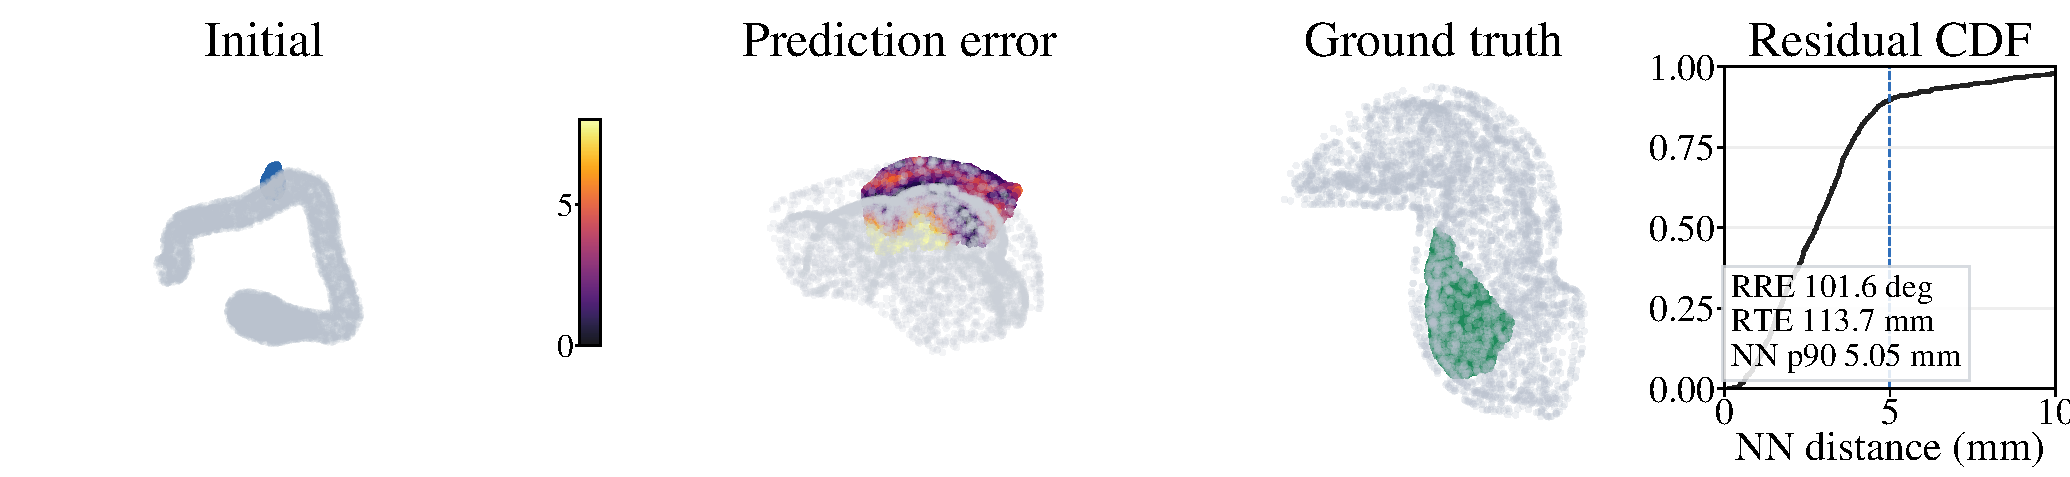
\includegraphics[width=\linewidth]{local_to_global_vs_raycast_target_row_01_scene_aligned_full_model.pdf}\\[-0.35em]
\figpanelleft{\linewidth}{(a) Local-to-global: full CT surface, sample A}
\end{minipage}
&
\begin{minipage}[t]{0.49\linewidth}
\centering
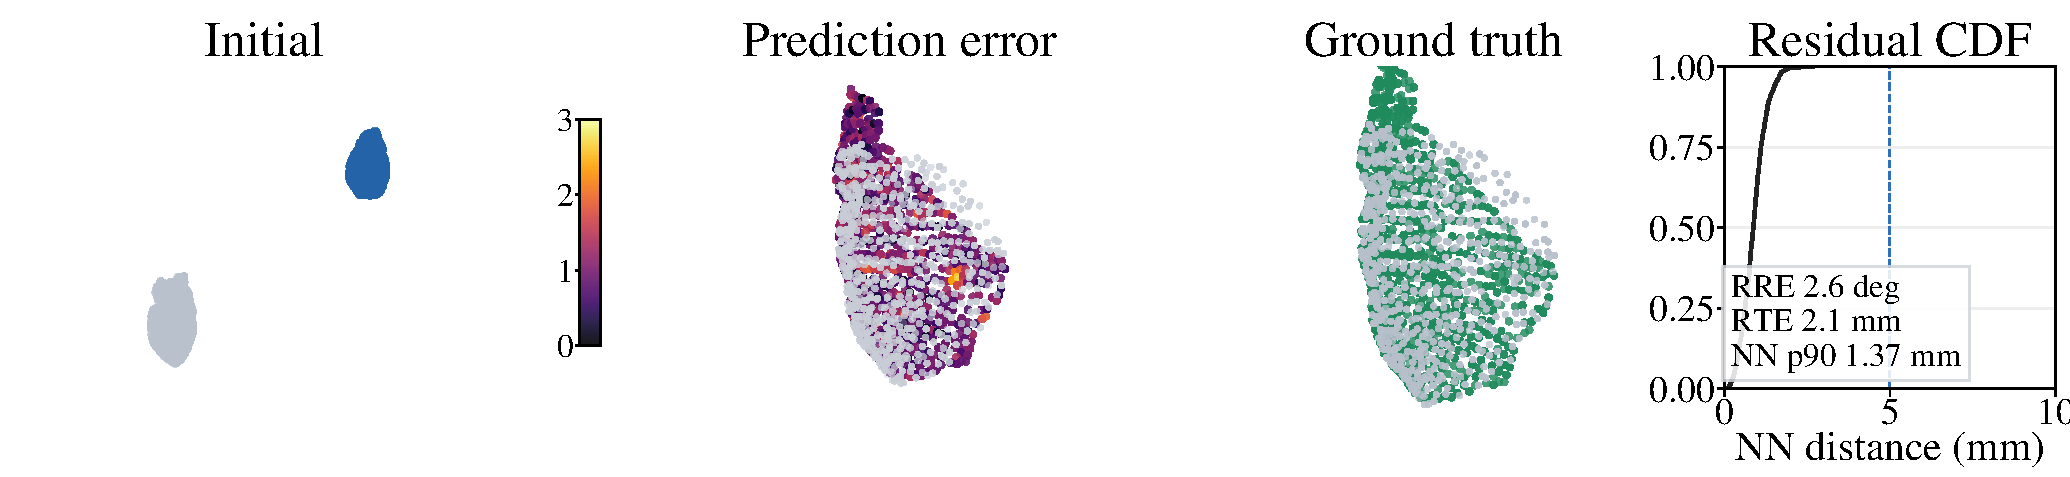
\includegraphics[width=\linewidth]{local_to_global_vs_raycast_target_row_02_frame_wise_raycast.pdf}\\[-0.35em]
\figpanelleft{\linewidth}{(b) Local-to-local: matched raycast CT surface, sample A}
\end{minipage}
\\[-0.05em]
\begin{minipage}[t]{0.49\linewidth}
\centering
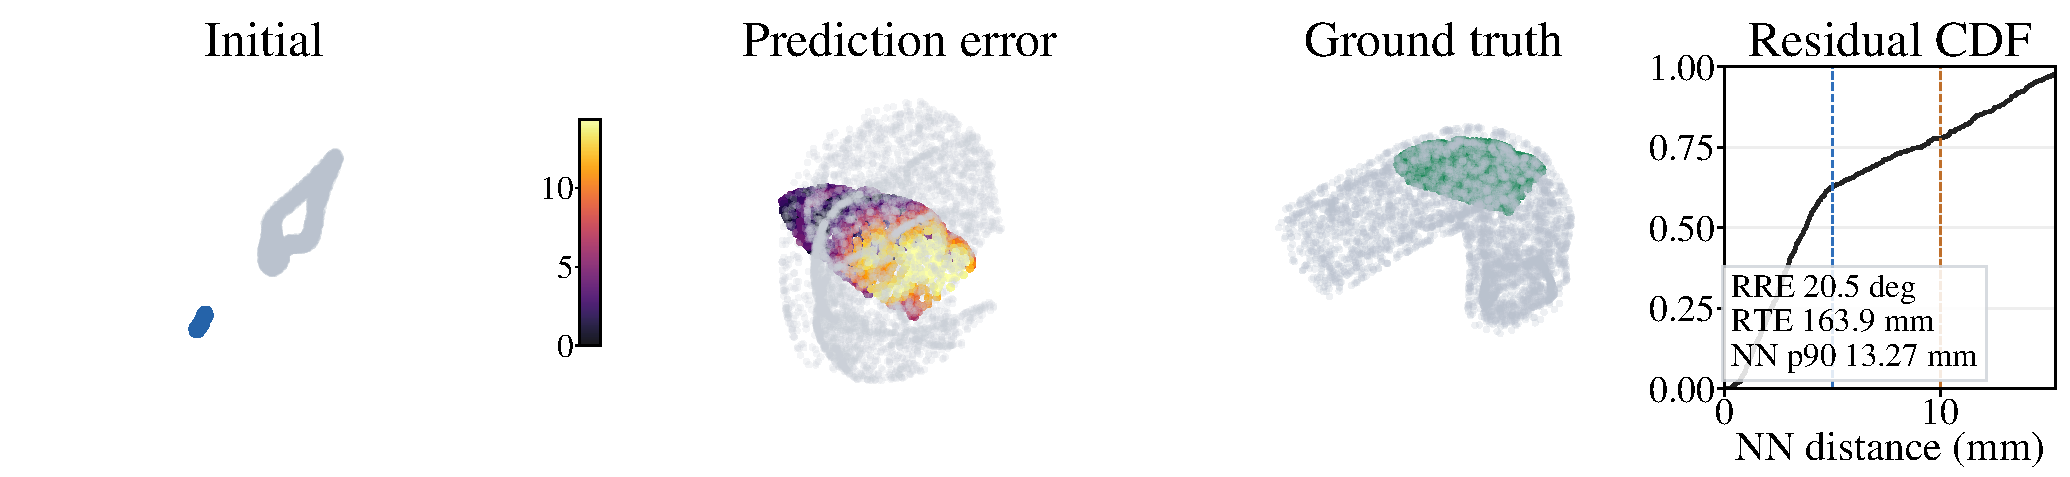
\includegraphics[width=\linewidth]{local_to_global_vs_raycast_target_row_03_scene_aligned_full_model.pdf}\\[-0.35em]
\figpanelleft{\linewidth}{(c) Local-to-global: full CT surface, sample B}
\end{minipage}
&
\begin{minipage}[t]{0.49\linewidth}
\centering
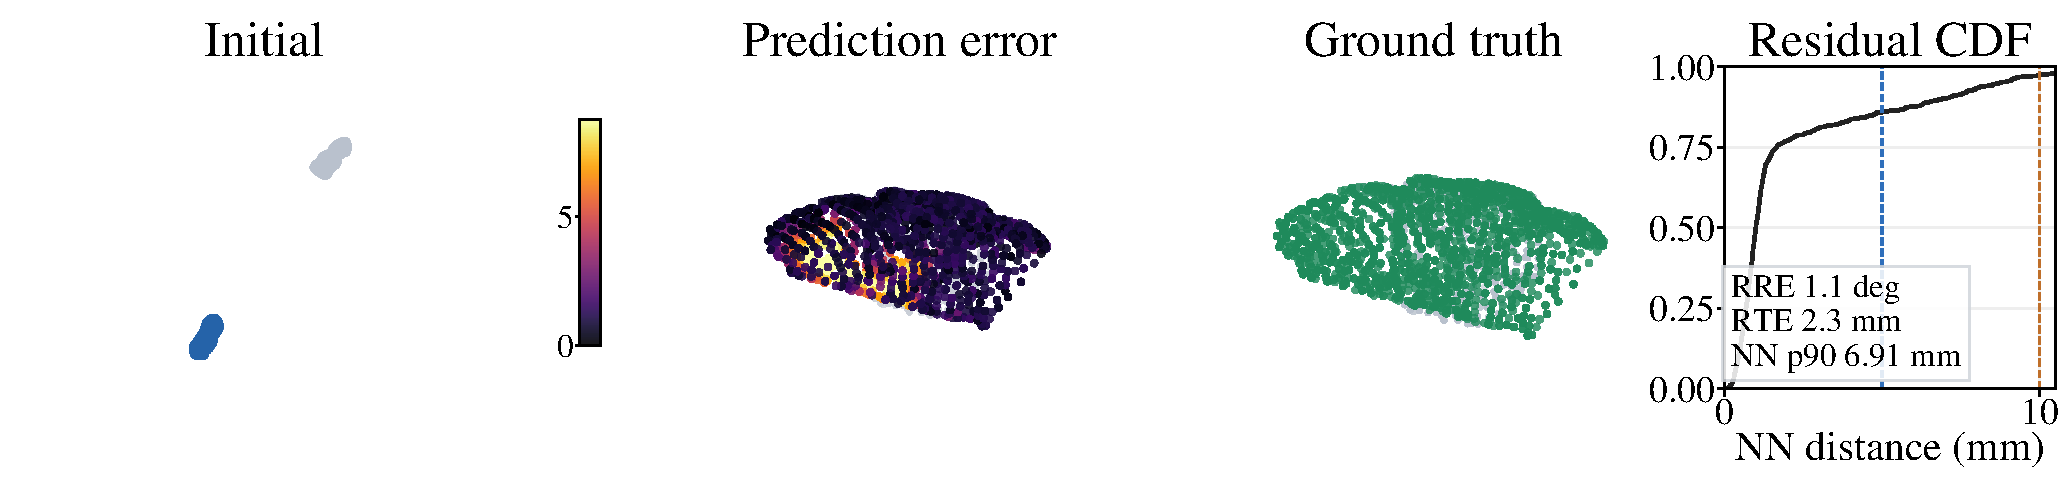
\includegraphics[width=\linewidth]{local_to_global_vs_raycast_target_row_04_frame_wise_raycast.pdf}\\[-0.35em]
\figpanelleft{\linewidth}{(d) Local-to-local: matched raycast CT surface, sample B}
\end{minipage}
\end{tabular}
\caption{Local-to-global diagnostic with GeoTransformer, the strongest baseline in the main C3VDReg benchmark. The same checkpoint is evaluated on identical source frames using either the full CT surface (local-to-global; a,c) or the matched raycast CT surface (local-to-local; b,d). The poorer full-surface results motivate C3VDReg as a controlled benchmark for local registration before full-surface localization.}
\label{fig:local_to_global_scope}
\end{figure*}

Figure~\ref{fig:local_to_global_scope} illustrates why this distinction matters. We apply GeoTransformer~\cite{qin2022geometric}, the best-performing baseline in our main experiments, to the same source frames under two target definitions. With the full CT surface as target, the method must perform local-to-global matching and the examples show severe pose errors. With the matched raycast surface as target, the visible CT region is specified and the same model achieves substantially better local alignment. The figure therefore motivates C3VDReg as an intermediate benchmark: before measuring full local-to-global colonoscopic localization, it is necessary to test whether current methods can reliably align corresponding local CT and video-depth observations.

Our experiments show that even this controlled setting remains unsolved. GeoTransformer is the strongest baseline, but reaches only 17.43\% strict Registration Recall at 5deg/5mm and 35.63\% at 10deg/10mm. Ground-truth overlap is already high after alignment, yet recall remains low and nonmonotonic across overlap quantiles. The dominant bottleneck is therefore not simply missing shared surface, but translation ambiguity caused by smooth and repetitive tubular anatomy.

Our contributions are:
\begin{enumerate}
    \item We introduce \textbf{C3VDReg}, a frame-wise registration benchmark and dataset with 10,015 viewpoint-matched partial-to-partial point-cloud pairs, generated from depth map reprojection and matched-pose CT mesh raycasting.
    \item We define a fixed benchmark contract with held out test scenes, an input budget of 8,192 points, R25--90deg/T100--500mm perturbations applied only to the source, a source-to-target pose convention, and explicit pose metrics.
    \item We evaluate representative classical and learning-based rigid registration baselines and show that translation ambiguity, not low visible overlap, is the main bottleneck for frame-wise colonoscopic registration; a full-surface diagnostic further shows that direct local-to-global matching remains substantially harder.
\end{enumerate}


\section{Related Work}
\label{sec:related}

\paragraph{Colonoscopy 3D datasets and benchmarks.}
Colonoscopy datasets have broadened the scope of computer vision research in this domain, but most focus on perception tasks other than rigid registration. C3VD is particularly important because it provides colonoscopy videos together with depth maps, camera poses, surface models, and coverage annotations, making it a natural foundation for geometry-aware evaluation~\cite{bobrow2023colonoscopy}. RealSynCol and SimCol3D target depth, pose, and reconstruction using synthetic or rendered supervision~\cite{lena2026realsyncol,rau2024simcol3d}, while REAL-Colon and SegCol focus on procedure-level analysis, polyp evaluation, fold-edge segmentation, and tool-aware perception~\cite{biffi2024realcolon,ju2024segcol}. These resources are clinically relevant and increasingly realistic, but they do not define a fixed benchmark contract for frame-wise rigid registration between video-derived partial observations and CT-derived colon anatomy. In particular, source/target construction, perturbation ranges, point budgets, pose conventions, and success metrics are generally left unspecified for this task.

\paragraph{Point cloud registration.}
Rigid point cloud registration spans classical geometric optimization and modern learning-based correspondence or pose estimation. ICP remains a standard local alignment baseline~\cite{besl1992method}. Learning-based approaches include iterative feature alignment methods such as PointNetLK and PointNetLK Revisited~\cite{aoki2019pointnetlk,li2021pointnetlk}, direct pose regression or correspondence learning such as DCP~\cite{wang2019deep}, and transformer-based registration methods such as RegTR and GeoTransformer~\cite{yew2022regtr,qin2022geometric}. Surveys have highlighted the broad range of assumptions these methods make about overlap, saliency, initialization, density, and scene structure~\cite{pomerleau2015review,huang2021comprehensive}. However, their empirical evaluation is dominated by CAD objects, indoor RGB-D fragments, and outdoor LiDAR scenes. Those benchmarks do not capture the geometry of colonoscopy, where observations are highly partial, surfaces are locally smooth yet strongly repetitive, and cross-domain differences arise between CT-derived anatomy and endoscopic depth reconstruction. Strong performance on general-purpose benchmarks therefore does not necessarily translate to robust colonoscopic registration.

\paragraph{Medical registration evaluation.}
Medical registration research has repeatedly emphasized that evaluation protocols should make modality assumptions, coordinate conventions, deformation assumptions, and clinically meaningful success criteria explicit~\cite{maier2013optical,haskins2020deep}. This is especially important in medical vision, where performance can change substantially depending on how correspondences are constructed, how initialization is sampled, and whether evaluation measures global pose recovery or only local geometric fit. C3VDReg follows this principle by fixing pair construction, source-to-target pose convention, perturbation distribution, point budget, and pose-based success metrics before evaluation. In this sense, our contribution is not a new registration algorithm, but a benchmark for a previously under-evaluated setting: rigid registration on tubular colon geometry with strong repetitive structure, enabling systematic comparison of classical and learning-based methods under one reproducible protocol.

\section{C3VDReg Dataset}
\label{sec:dataset}

\subsection{Pair Construction}
\label{sec:pair_construction}

C3VDReg is derived from released C3VD assets and introduces no new human subject data collection. C3VD provides colonoscopy videos, depth maps, camera poses, and CT surface meshes~\cite{bobrow2023colonoscopy}. We use these assets to construct deterministic frame-wise registration artifacts: source clouds from video depth, target clouds from CT mesh visibility, fixed splits, and evaluation metadata.

Each registration pair is built from two matched but distinct C3VD data streams. The source point cloud $P_S$ comes from the released colonoscopic depth frame: valid pixels are unprojected with the camera intrinsics and then transformed into the global C3VD coordinate frame.

The target point cloud $P_T$ is generated from the C3VD CT mesh by placing a virtual camera at the same released pose, as summarized in Figure~\ref{fig:dataset_construction}. Here a CT mesh is the triangulated anatomical surface reconstructed from CT, and raycasting means intersecting each virtual camera ray with that mesh. For each image plane sample, the nearest mesh intersection along the camera line of sight is computed with the Moller--Trumbore algorithm~\cite{moller1997fast} and retained to model the visible anatomical surface. The pair is viewpoint-matched but drawn from different measurement sources, so the task remains a registration problem between partial clouds with a density mismatch before the source perturbation is applied.

\begin{figure*}[t]
    \centering
    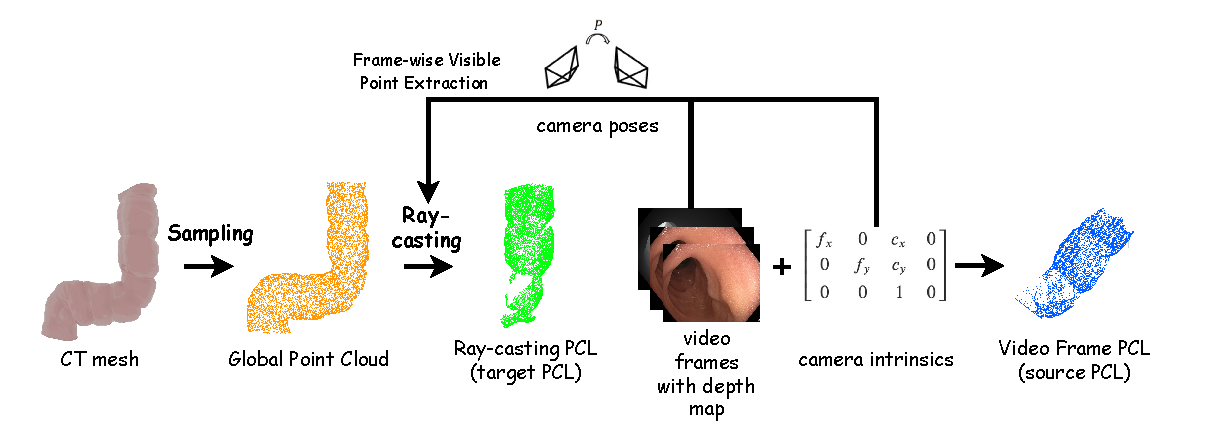
\includegraphics[width=\textwidth]{c3vd_raycasting.pdf}
    \caption{Frame-wise C3VDReg pair construction. For each C3VD frame, the source point cloud is generated by reprojecting the released depth map with camera intrinsics and pose. The target point cloud is generated by placing a virtual camera at the matched pose and raycasting the CT mesh to extract the visible anatomical surface. This creates viewpoint-matched partial-to-partial pairs while leaving full local-to-global retrieval outside the benchmark scope.}
    \label{fig:dataset_construction}
\end{figure*}

C3VDReg should therefore be interpreted as a controlled intermediate benchmark toward clinical local-to-global colonoscopic registration. The raycast target provides the oracle visible CT surface: it isolates frame-wise rigid partial-to-partial alignment once the corresponding visible CT region is specified, but it does not solve full mesh localization, viewpoint mismatch, or deformation.

\subsection{Splits and Release}
\label{sec:splits}

C3VDReg contains 10,015 generated pairs, split into 5,952 train pairs, 1,975 validation pairs, and 2,088 test pairs. The full test split is drawn from six held out scenes: \texttt{cecum\_t1\_a} (276), \texttt{cecum\_t3\_a} (730), \texttt{sigmoid\_t3\_b} (536), \texttt{trans\_t1\_a} (61), \texttt{trans\_t2\_b} (103), and \texttt{trans\_t4\_a} (382). Held out scenes test anatomy generalization more directly than a random pair split.

The release is intended to provide pair manifests, split files, generation scripts, evaluation scripts, and baseline configuration templates.\footnote{\url{https://doi.org/10.5522/04/30640043}} Redistribution of derived point clouds should follow the upstream C3VD terms.

\section{Benchmark Definition}
\label{sec:benchmark_definition}
\label{sec:protocol}

The evaluation protocol is specified before training and evaluation. Each method receives a perturbed source cloud and a target cloud, and predicts the rigid source to target transformation. All main results use the same point budget, perturbation distribution, pose convention, and metric suite to prevent method specific preprocessing or split choices from changing the task. Table~\ref{tab:protocol} summarizes this contract.

\begin{table}[t]
\centering
\caption{Fixed C3VDReg evaluation contract used by all main experiments. The table defines the data split, point budget, perturbation range, pose convention, primary recalls, geometry diagnostics, and runtime diagnostic.}
\label{tab:protocol}
\small
\begin{tabular}{ll}
\hline
Item & Main protocol \\
\hline
Dataset source & C3VDReg \\
Task & Rigid registration between partial source and target clouds \\
Manifest & 10,015 pairs: 5,952 train, 1,975 val, 2,088 test \\
Test scenes & Six held out C3VD scenes \\
Input points & 8,192 source points and 8,192 target points \\
Perturbation & R25--90deg/T100--500mm applied only to source, no added noise \\
Primary recall & RR@5 and RR@10, defined at 5deg/5mm and 10deg/10mm \\
Error metrics & RRE in degrees, RTE in mm \\
Geometry diagnostics & Visible NN and trimmed Chamfer distance in mm \\
Runtime diagnostic & Pair latency under the shared point budget \\
\hline
\end{tabular}
\end{table}

\paragraph{Metrics.}
\label{sec:metrics}

All predictions and ground truth use the source to target convention. We evaluate global pose accuracy with relative rotation error (RRE), the geodesic angle between predicted and ground truth rotations, and relative translation error (RTE), the Euclidean translation error in millimetres. Registration Recall at strict thresholds, abbreviated RR@5 in tables, is the percentage of pairs with RRE no larger than 5deg and RTE no larger than 5mm; RR@10 uses 10deg and 10mm. We also report marginal rotation and translation hit rates, denoted R$\leq$5 and T$\leq$5, to separate rotation recovery from translation recovery.

Mean errors summarize average performance, while medians and 90th percentiles expose typical and tail behavior. An empirical cumulative distribution function (empirical CDF) plots, for each error threshold on the $x$ axis, the fraction of evaluated pairs whose error is at or below that threshold. We do not report target registration error (TRE), because the benchmark has no independent landmark targets. Geometry diagnostics are computed after applying the predicted transform: visible nearest neighbor (NN) distance is the Euclidean distance from a transformed source point to its closest target point, and 90\% trimmed Chamfer removes the largest residuals before computing bidirectional distance. In qualitative figures, a residual CDF is the same cumulative plot applied to these pointwise NN residual distances within one pair. These residual metrics describe local fit, but they do not replace global pose accuracy.

For prediction independent stratification, we compute symmetric GT overlap after applying the ground truth transform. A source or target point is counted as overlapping if its nearest neighbor in the opposite cloud is within 5mm. The final score averages the source to target and target to source fractions, and is used only to stratify the fixed test set.

Runtime columns use the same point budget for all methods. Pre. is preprocessing time, Infer is prediction time, Latency is their sum, and Lat. 90th pct. is the latency value below which 90\% of evaluated pairs finish. Eval res. and Eval alloc. are CUDA peak reserved and allocated memory during standardized batch size one prediction calls. Runtime is treated as a diagnostic rather than a primary success criterion, because the central benchmark question is whether a method recovers the source to target pose under strict RRE/RTE thresholds.

In comparable metric columns, bold marks the best value and underline marks the second best value; noncomparative, categorical, or constant columns are left unranked.

\paragraph{Baselines.}
\label{sec:baseline_initialization}

We evaluate representative methods from major registration families under the fixed C3VDReg contract: classical geometry (ICP~\cite{besl1992method}), sparse feature matching (GeoTransformer~\cite{qin2022geometric} and RegTR~\cite{yew2022regtr}), LK family methods (PointNetLK~\cite{aoki2019pointnetlk}, PointNetLK Revisited~\cite{li2021pointnetlk}, and PointNetLK-Mamba), and DCP~\cite{wang2019deep}. ICP is included as a classical reference baseline evaluated on CPU rather than as a trained method. All baselines are evaluated under the same split, point budget, perturbation, pose convention, and metric suite.

\section{Technical Validation and Benchmark Results}
\label{sec:experiments}

The analysis evaluates whether failures are primarily caused by insufficient shared surface. If this explanation were correct, methods should become reliable on pairs with high GT overlap. The fixed protocol allows us to test this explanation without changing the task. We first separate rotation and translation errors, then stratify by overlap, and finally relate the remaining translation tail to tubular geometric ambiguity.

\subsection{The Translation Bottleneck in Colonoscopic Registration}
\label{sec:main_results}

First, current public methods fail on a large fraction of test pairs. Under the fixed C3VDReg contract, no method reaches a reliable recall level. Aggregate recall gives the overall result, but it is not sufficient on its own: a method may recover orientation while losing position, or succeed on a small subset while producing large errors on the remaining cases.

\begin{table*}[t]
\centering
\caption{Main leaderboard for the fixed C3VDReg protocol with R25--90deg/T100--500mm perturbations applied only to the source. RR@5 and RR@10 denote joint Registration Recall at 5deg/5mm and 10deg/10mm, respectively. Even the strongest method satisfies the strict threshold for fewer than one in five test pairs.}
\label{tab:main_results}
\scriptsize
\setlength{\tabcolsep}{3.2pt}
\begin{tabular}{lrrrrrrr}
\hline
Model & RR@5 & RR@10 & RRE mean & RTE mean & Visible NN & Trim CD & Latency \\
 & (\%) & (\%) & (deg) & (mm) & (mm) & (mm) & (ms) \\
\hline
GeoTransformer~\cite{qin2022geometric} & \best{17.43} & \best{35.63} & \best{10.79} & \best{44.22} & \best{1.49} & \best{2.42} & 186.8 \\
ICP~\cite{besl1992method} & \second{5.46} & 10.73 & 54.62 & 217.21 & 3.15 & 3.89 & 787.7 \\
RegTR~\cite{yew2022regtr} & 5.32 & \second{11.59} & 32.33 & 133.01 & 5.58 & 6.16 & \second{83.0} \\
PointNetLK-Mamba & 3.16 & 11.11 & \second{18.17} & \second{74.15} & 3.05 & \second{3.52} & 121.7 \\
PointNetLK Revisited~\cite{li2021pointnetlk} & 2.39 & 10.58 & 30.62 & 119.22 & \second{2.97} & 3.69 & 132.1 \\
PointNetLK~\cite{aoki2019pointnetlk} & 0.14 & 1.01 & 47.07 & 194.70 & 4.81 & 5.82 & 93.1 \\
DCP~\cite{wang2019deep} & 0.00 & 0.00 & 84.15 & 313.21 & 13.51 & 18.17 & \best{64.3} \\
\hline
\end{tabular}
\end{table*}

Table~\ref{tab:main_results} shows that the protocol is not saturated. GeoTransformer leads, but 17.43\% RR@5 and 35.63\% RR@10 leave most test pairs outside the success thresholds. ICP serves as a local reference baseline, yet its much larger mean RRE/RTE indicates that its successes are limited to a small convergent subset. DCP is the fastest method but has no strict-threshold successes, showing that speed alone does not imply robustness under these large perturbations between partial colonoscopic clouds.

The aggregate leaderboard also obscures which part of the pose is failing. Table~\ref{tab:error_distribution} separates marginal rotation and translation hits from joint recall: GeoTransformer places 56.18\% of pairs within 5deg rotation error, but only 18.15\% within 5mm translation error. Strict RR@5 is limited by translation. ICP reaches 114/2088 strict RR@5 successes, but its median and 90th percentile RTE are 123.72mm and 570.22mm, respectively. This recall therefore reflects local convergence on a small subset rather than global robustness.

\begin{table}[!htbp]
\centering
\caption{Marginal and distributional error diagnostics for the main protocol. R$\leq$5 and T$\leq$5 are rotation only and translation only hit rates; RR@5 requires both. The large gap between GeoTransformer's rotation and translation hit rates identifies translation as the main bottleneck.}
\label{tab:error_distribution}
\scriptsize
\setlength{\tabcolsep}{3.4pt}
\begin{tabular}{lrrrrrrr}
\hline
Model & R$\leq$5 & T$\leq$5 & RR@5 & RTE med. & RTE 90th pct. & RRE med. & RRE 90th pct. \\
 & (\%) & (\%) & (\%) & (mm) & (mm) & (deg) & (deg) \\
\hline
GeoTransformer~\cite{qin2022geometric} & \best{56.18} & \best{18.15} & \best{17.43} & \best{15.86} & \best{82.12} & \best{4.29} & \best{17.16} \\
ICP~\cite{besl1992method} & 21.12 & \second{5.70} & \second{5.46} & 123.72 & 570.22 & 35.56 & 138.29 \\
RegTR~\cite{yew2022regtr} & 18.87 & 5.41 & 5.32 & 72.81 & 335.76 & 19.84 & 78.92 \\
PointNetLK-Mamba & 24.28 & 3.64 & 3.16 & 39.47 & \second{174.23} & 10.61 & \second{37.87} \\
PointNetLK Revisited~\cite{li2021pointnetlk} & \second{30.32} & 2.78 & 2.39 & \second{34.62} & 374.88 & \second{7.40} & 106.41 \\
PointNetLK~\cite{aoki2019pointnetlk} & 2.73 & 0.19 & 0.14 & 154.89 & 413.49 & 43.02 & 87.17 \\
DCP~\cite{wang2019deep} & 0.00 & 0.00 & 0.00 & 279.08 & 565.08 & 72.95 & 155.14 \\
\hline
\end{tabular}
\end{table}

Figure~\ref{fig:main_curves} shows the same trend at finer granularity. Scene recall is concentrated in particular held out anatomy rather than distributed evenly. GeoTransformer reaches 63.04\% RR@5 in \texttt{cecum\_t1\_a}, but only 0.93\% in \texttt{sigmoid\_t3\_b}. The empirical CDFs explain the leaderboard: RRE is often moderate for the strongest learned methods, while RTE retains a long tail. In this benchmark, the main difficulty is localization rather than orientation.

\begin{figure*}[!t]
\centering
\setlength{\tabcolsep}{2pt}
\begin{tabular}{cc}
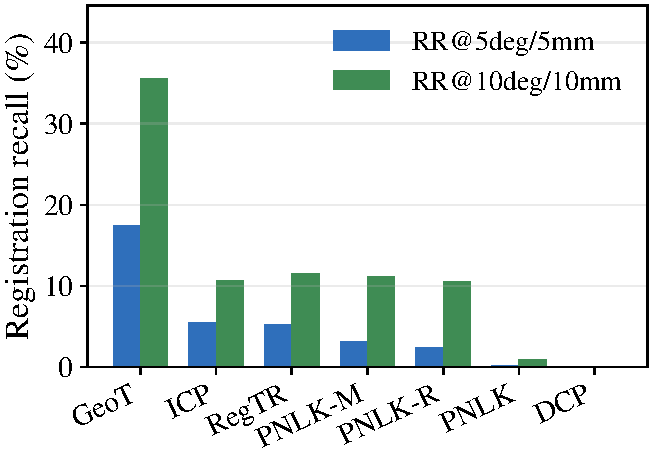
\includegraphics[width=0.48\textwidth]{images/hard_main_rr_bar.pdf} &
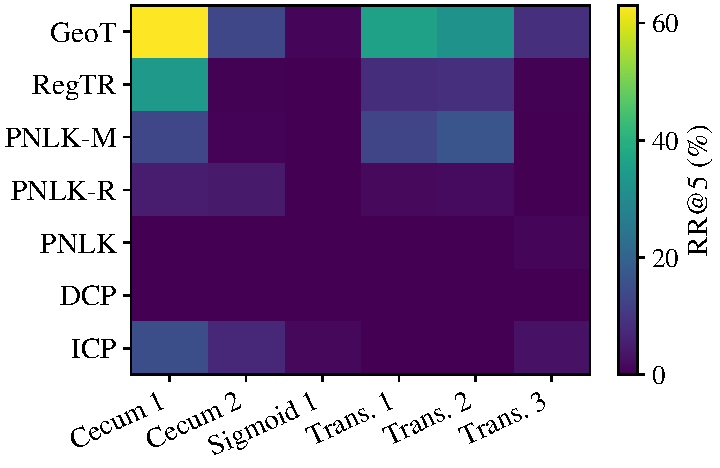
\includegraphics[width=0.48\textwidth]{images/hard_scene_bucket_rr.pdf} \\
\figpanel{0.48\textwidth}{(a) Strict registration recall} &
\figpanel{0.48\textwidth}{(b) Scene RR@5deg/5mm} \\[0.35em]
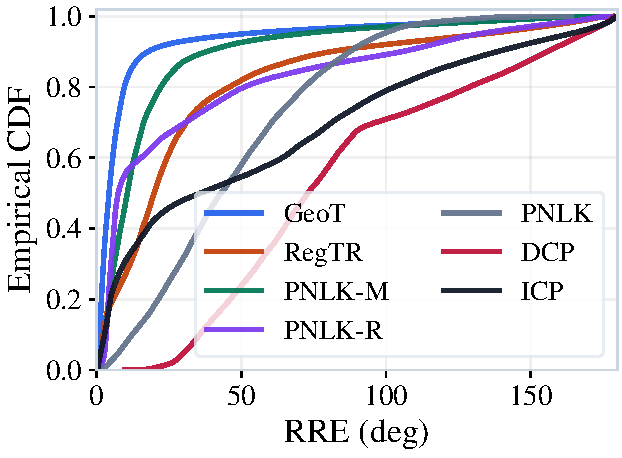
\includegraphics[width=0.48\textwidth]{images/hard_rre_cdf.pdf} &
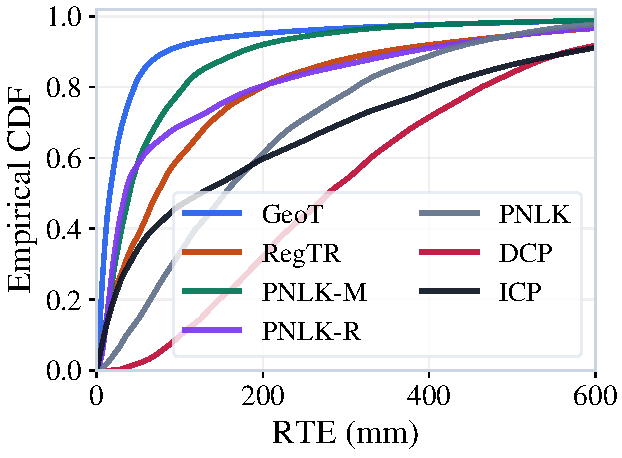
\includegraphics[width=0.48\textwidth]{images/hard_rte_cdf.pdf} \\
\figpanel{0.48\textwidth}{(c) RRE empirical CDF} &
\figpanel{0.48\textwidth}{(d) RTE empirical CDF}
\end{tabular}
\caption{Main benchmark views. (a) Joint recall at 5deg/5mm and 10deg/10mm thresholds. (b) Scene RR@5 across held out scenes shows strong anatomy dependence. (c,d) Empirical CDFs of RRE and RTE; at any error threshold, the curve height is the fraction of test pairs below that error. Translation errors have substantially longer tails than rotation errors.}
\label{fig:main_curves}
\end{figure*}

\subsection{Decoupling Failure from Geometric Overlap}
\label{sec:error_analysis}

A natural explanation for large translation errors is that the source and target might share too little visible surface. We test this directly with a prediction-independent GT overlap score. For each fixed test pair, we join per pair results by \texttt{sample\_id} and compute symmetric GT overlap after applying the ground truth transform, using a 5mm radius and 2048 deterministic points per cloud.

\begin{table*}[t]
\centering
\begin{minipage}[t]{0.49\textwidth}
\centering
\caption{GT-overlap quantiles. RR@5 remains nonmonotonic despite high overlap; GeoT RTE is in mm.}
\label{tab:overlap_quantiles}
\scriptsize
\setlength{\tabcolsep}{1.5pt}
\begin{tabular}{@{}lrrrrr@{}}
\hline
GT overlap & \shortstack{GeoT\\[-0.15em]\cite{qin2022geometric}} & \shortstack{RegTR\\[-0.15em]\cite{yew2022regtr}} & \shortstack{ICP\\[-0.15em]\cite{besl1992method}} & PNLK-M & GeoT RTE \\
quantile & RR@5 & RR@5 & RR@5 & RR@5 & 90th pct. \\
\hline
Q1 74.3--78.1\% & \second{12.45} & 0.19 & \second{8.05} & 0.57 & 141.68 \\
Q2 78.1--83.8\% & 12.07 & \second{1.72} & 4.21 & \second{2.30} & 123.48 \\
Q3 83.8--87.8\% & \best{37.16} & \best{17.82} & \best{8.62} & \best{8.43} & \best{52.16} \\
Q4 87.9--93.1\% & 8.05 & 1.53 & 0.96 & 1.34 & \second{65.81} \\
\hline
\end{tabular}
\end{minipage}
\hfill
\begin{minipage}[t]{0.49\textwidth}
\centering
\caption{Axial/radial translation tails. Radial 90th percentile error exceeds axial error for every learned method.}
\label{tab:axial_radial}
\scriptsize
\setlength{\tabcolsep}{4.2pt}
\begin{tabular}{lrr}
\hline
Model & Axial & Radial \\
 & 90th pct. & 90th pct. \\
 & (mm) & (mm) \\
\hline
GeoT~\cite{qin2022geometric} & \best{42.62} & \best{64.77} \\
PNLK-M & \second{75.33} & \second{146.41} \\
RegTR~\cite{yew2022regtr} & 177.36 & 268.62 \\
PNLK-R~\cite{li2021pointnetlk} & 193.87 & 278.22 \\
PNLK~\cite{aoki2019pointnetlk} & 232.38 & 337.41 \\
DCP~\cite{wang2019deep} & 345.10 & 478.99 \\
\hline
\end{tabular}
\end{minipage}
\end{table*}

Table~\ref{tab:overlap_quantiles} argues against low overlap as the primary explanation in this protocol. All 2,088 test pairs have high overlap after GT alignment: the four equal size quantiles span 74.3--78.1\%, 78.1--83.8\%, 83.8--87.8\%, and 87.9--93.1\%. Yet Figure~\ref{fig:overlap_and_tail}(a) shows that strict RR@5 is nonmonotonic. GeoTransformer and RegTR improve in Q3 but fall again in Q4, while DCP remains at zero strict recall across all quantiles. High visible surface overlap by itself does not guarantee millimetre scale global translation recovery.

\begin{figure*}[t]
\centering
\setlength{\tabcolsep}{2pt}
\begin{tabular}{cc}
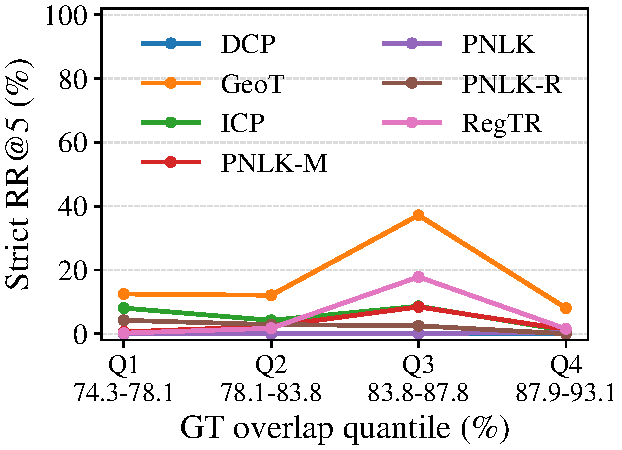
\includegraphics[width=0.48\linewidth]{hard_overlap_quantile_rr_curve.pdf} &
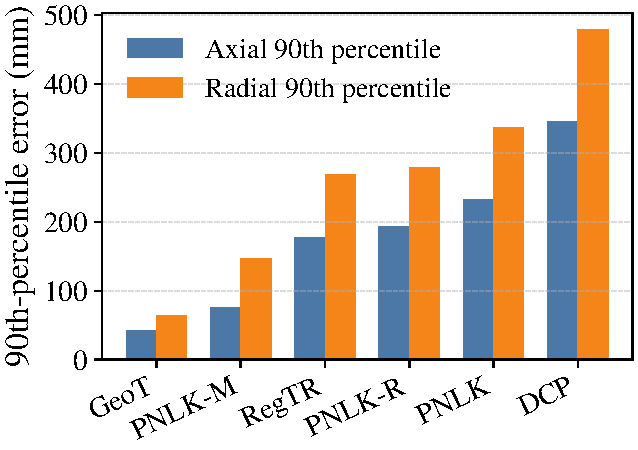
\includegraphics[width=0.48\linewidth]{hard_axial_radial_translation_p90.pdf} \\
\figpanel{0.48\linewidth}{(a) Strict RR@5 by GT overlap quantile} &
\figpanel{0.48\linewidth}{(b) Axial/radial translation tails}
\end{tabular}
\caption{Overlap and translation tail diagnostics. (a) Strict RR@5 is nonmonotonic across high overlap GT quantiles, arguing against missing shared surface as the dominant explanation. (b) Learned baselines retain large axial and radial translation tails, indicating both sliding along the trajectory and cross-trajectory errors.}
\label{fig:overlap_and_tail}
\label{fig:overlap_quantile_rr}
\label{fig:axial_radial}
\end{figure*}

\subsection{Geometric Ambiguity: The Illusion of Local Fit}
\label{sec:axial_radial}
\label{sec:qualitative}

We next examine the source of the translation tail. A plausible anatomical failure mode is axial sliding along the colon trajectory: the model aligns a nearby tubular segment but shifts forward or backward along the lumen. We test this by decomposing each learned baseline's translation error vector into trajectory axial and radial components. The axial error is the absolute projection of the translation error onto the local trajectory direction, and the radial error is the remaining orthogonal magnitude. The axial direction is estimated from neighboring C3VD camera centers, so it is a trajectory-derived centerline proxy rather than a manually annotated anatomical centerline. ICP is omitted from this post hoc decomposition because the saved CPU evaluation outputs did not include per pair transforms; its main metrics remain in Tables~\ref{tab:main_results} and~\ref{tab:error_distribution}.

The decomposition in Figure~\ref{fig:overlap_and_tail}(b) and Table~\ref{tab:axial_radial} shows that axial sliding is only part of the failure. GeoTransformer has the smallest component tails, yet its axial and radial 90th percentile errors are still 42.62mm and 64.77mm. For every learned method, the radial 90th percentile exceeds the axial 90th percentile. Under strong source perturbations, learned baselines therefore exhibit both trajectory sliding and cross-trajectory mislocalization.

Quantitative metrics show that local residuals and global pose accuracy can diverge, so we use GeoTransformer, the strongest baseline in C3VDReg, for a focused qualitative check. Figure~\ref{fig:qualitative} keeps two cases: a low residual mismatch, where the residual map/CDF looks locally plausible despite a wrong global pose, and a high residual failure, where local fit and pose accuracy are both poor.

\begin{figure*}[tbp]
\centering
\setlength{\tabcolsep}{0pt}
\begin{tabular}{c}
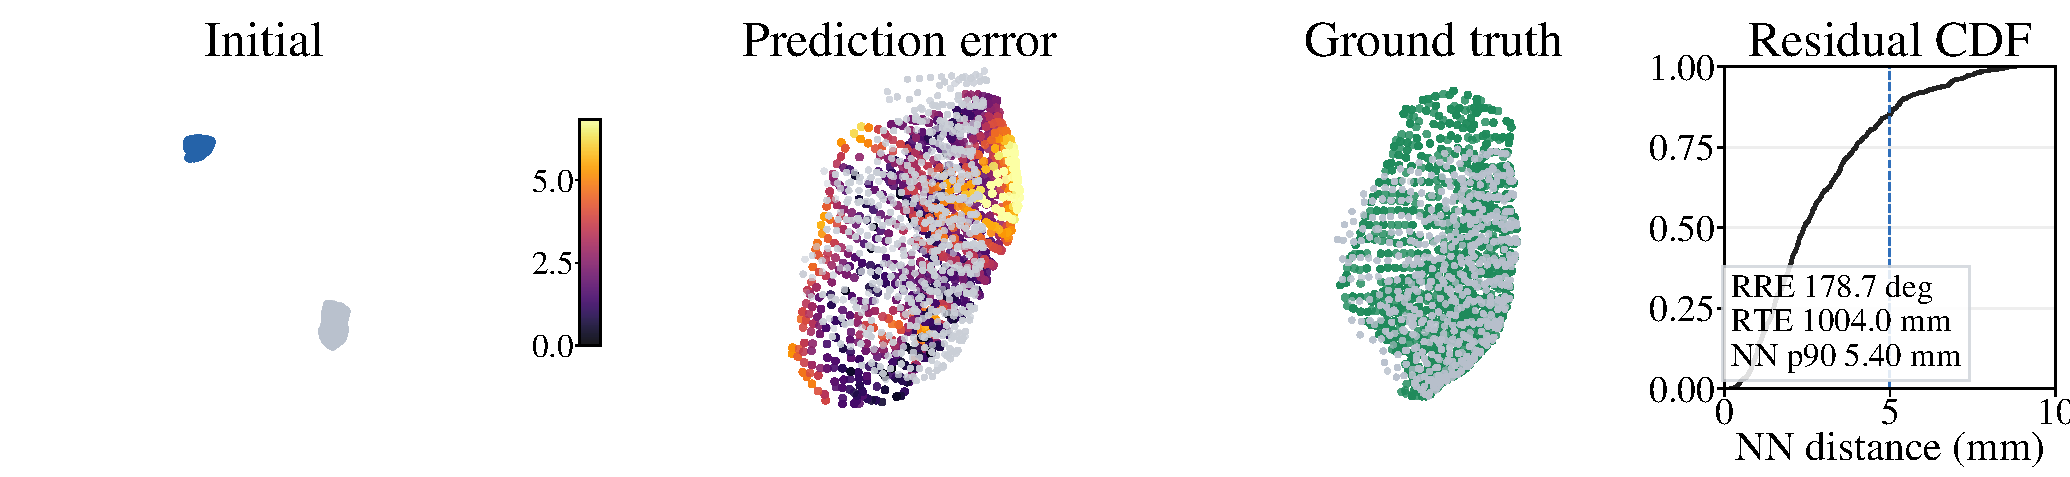
\includegraphics[width=\linewidth]{geotransformer_failure_cases_row_01.pdf}\\[-0.30em]
\figpanelleft{\linewidth}{(a) Low residual mismatch: NN p90 5.40 mm, RTE 1004.0 mm}\\[-0.10em]
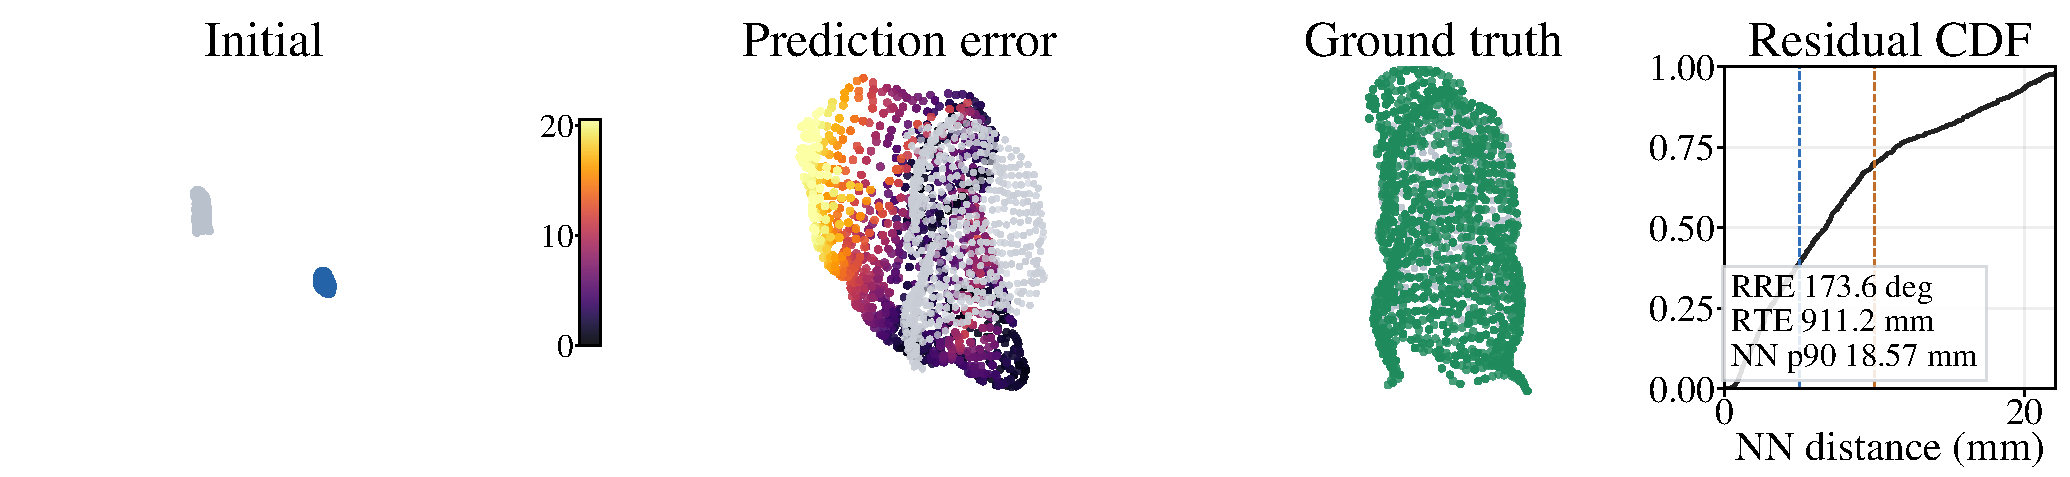
\includegraphics[width=\linewidth]{geotransformer_failure_cases_row_05.pdf}\\[-0.30em]
\figpanelleft{\linewidth}{(b) High residual failure: NN p90 18.57 mm, RTE 911.2 mm}
\end{tabular}
\caption{Two GeoTransformer failure regimes under C3VDReg. Columns show the initial pair, prediction error map, ground truth alignment, and residual CDF. Row (a) has low local residuals despite a globally wrong pose; row (b) has both high residuals and large pose error.}
\label{fig:qualitative}
\end{figure*}

The distinction is diagnostic rather than a taxonomy of all failures. The low residual case shows why residual only evaluation is insufficient: repeated tubular wall geometry can make a displaced patch look locally plausible. The high residual case is the conventional failure in which residuals and pose metrics agree. Together, the cases explain why C3VDReg reports pose metrics as the primary endpoint and uses residual distances as supporting diagnostics.

\begin{figure*}[!t]
\centering
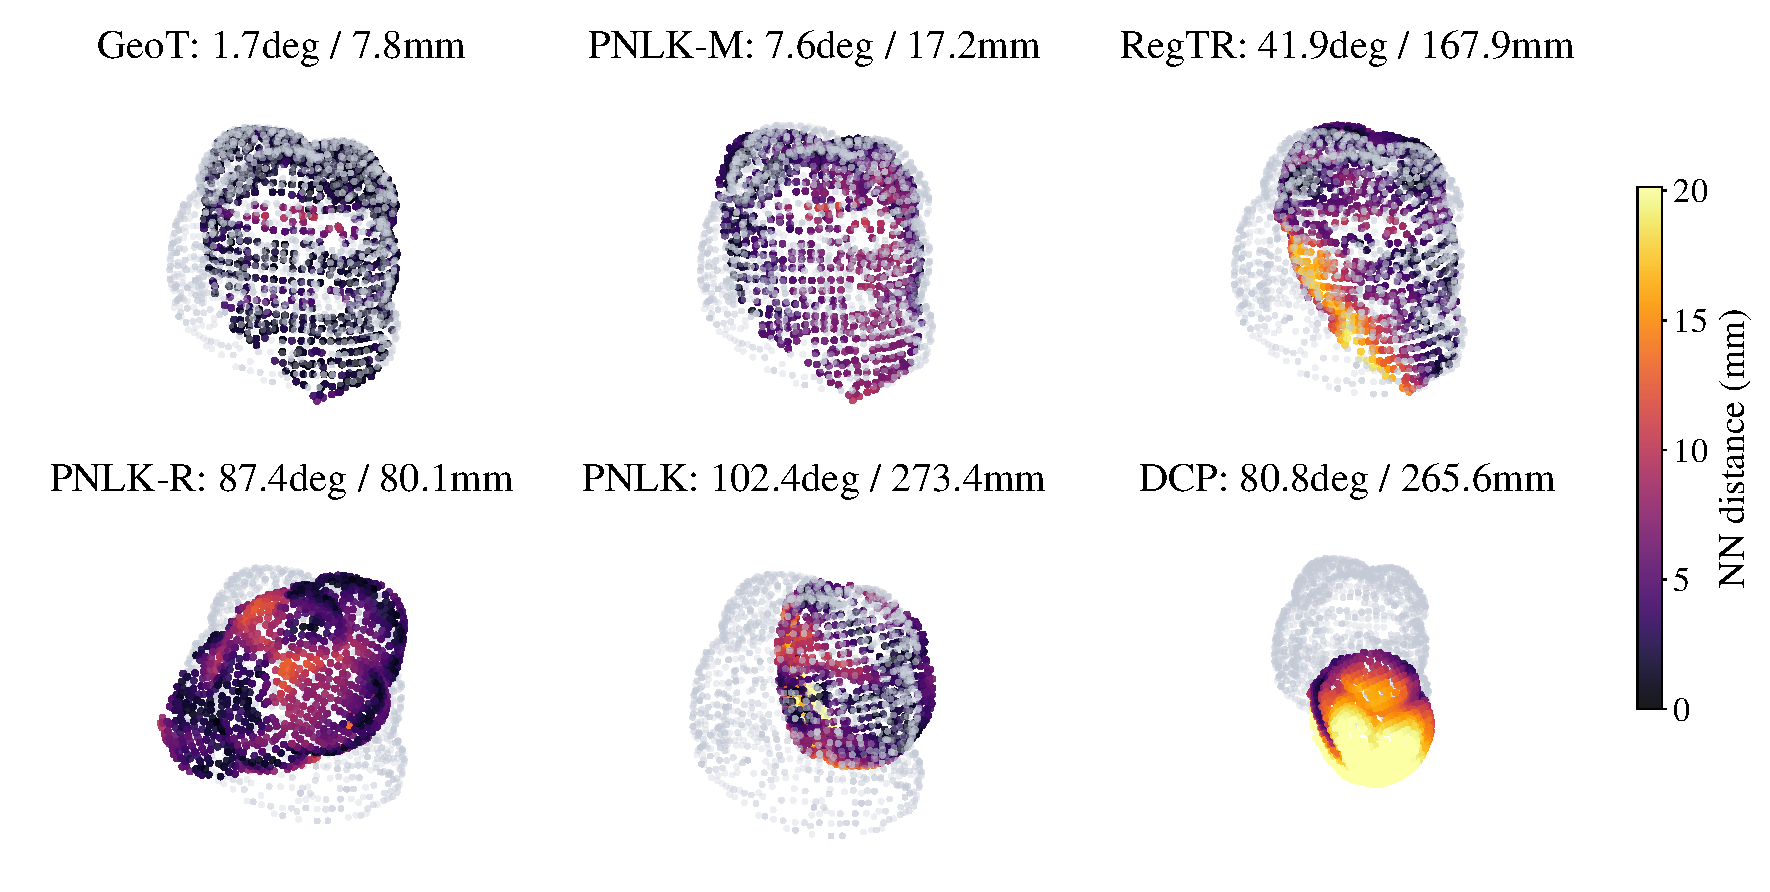
\includegraphics[width=\textwidth]{same_sample_model_comparison.pdf}
\caption{Same sample model comparison on \texttt{cecum\_t3\_a:0133}. Target points are gray and predicted source points are colored by nearest neighbor residual with a shared scale. GeoTransformer is closest on this sample, PNLK-M remains close, while RegTR, PNLK-R, PNLK, and DCP drift farther on the same input.}
\label{fig:same_sample_comparison}
\end{figure*}

Figure~\ref{fig:same_sample_comparison} connects the aggregate failure analysis to a single fixed test pair. Its visual ordering mirrors the translation tail ordering in Figure~\ref{fig:overlap_and_tail}(b): GeoTransformer is closest, PointNetLK-Mamba (PNLK-M in the figure) is the next closest, RegTR is visibly worse, and PointNetLK Revisited, PointNetLK, and DCP drift farther on the same input. This agreement provides qualitative support that the axial/radial tail metric reflects visible differences in global alignment quality, rather than acting only as a summary statistic.

The comparison also illustrates why model quality should not be judged by strict recall alone. RR@5 is essential because it measures whether both rotation and translation meet a deployment relevant tolerance, but it is a thresholded binary statistic: it does not distinguish a near miss from a large drift once both fail the threshold. For example, RegTR has higher RR@5 than PointNetLK-Mamba in Table~\ref{tab:main_results}, but Table~\ref{tab:axial_radial} and Figure~\ref{fig:same_sample_comparison} show that PointNetLK-Mamba has smaller translation tails and a less severe drift on the same pair. The benchmark should be interpreted jointly through recall, RRE/RTE distributions, axial/radial tails, residual maps, and qualitative alignment, rather than using recall alone for model selection.

\subsection{The Robustness and Efficiency Tradeoff}
\label{sec:efficiency}

The preceding sections characterize the geometric failure mode; runtime analysis captures the practical computational constraint. Colonoscopic navigation systems are naturally online or near online, so an effective architecture must be both robust to tubular ambiguity and computationally feasible. Combining Table~\ref{tab:main_results} with Table~\ref{tab:efficiency} shows that the evaluated methods do not yet satisfy both requirements: DCP is the fastest learned baseline at 64.3ms but has no strict-threshold successes, RegTR is faster than GeoTransformer but has much lower recall, GeoTransformer is the most robust but slower, and ICP is CPU only and substantially slower.

\begin{table}[!htbp]
\centering
\caption{Runtime and memory profile under the fixed main protocol. Timings are pairwise evaluation costs and memory columns report standardized batch size one CUDA peaks. The fastest learned baseline has zero strict recall, whereas the strongest baseline has higher latency, indicating an accuracy--efficiency trade-off under the current protocol.}
\label{tab:efficiency}
\scriptsize
\setlength{\tabcolsep}{3.5pt}
\begin{tabular}{lrrrrrrrr}
\hline
Model & Input & Train & Eval res. & Eval alloc. & Pre. & Infer & Latency & Lat. 90th pct. \\
 & pts & h/ep & MB & MB & ms & ms & ms & ms \\
\hline
GeoTransformer~\cite{qin2022geometric} & 8192 & 0.086 & \best{484.0} & \best{396.8} & \second{4.8} & 182.0 & 186.8 & 267.1 \\
ICP~\cite{besl1992method} & 8192 & -- & -- & -- & 5.0 & 782.8 & 787.7 & 946.3 \\
RegTR~\cite{yew2022regtr} & 8192 & 0.228 & \second{508.0} & 423.2 & \best{4.7} & \second{78.3} & \second{83.0} & 118.6 \\
PointNetLK-Mamba & 8192 & 0.026 & 1396.0 & 756.8 & \best{4.7} & 117.0 & 121.7 & 155.2 \\
PointNetLK Revisited~\cite{li2021pointnetlk} & 8192 & \second{0.024} & 8960.0 & 8761.6 & \second{4.8} & 127.4 & 132.1 & 162.9 \\
PointNetLK~\cite{aoki2019pointnetlk} & 8192 & \best{0.004} & 516.0 & \second{405.7} & \second{4.8} & 88.4 & 93.1 & \second{116.0} \\
DCP~\cite{wang2019deep} & 8192 & 0.324 & 6180.0 & 5341.6 & \second{4.8} & \best{59.4} & \best{64.3} & \best{67.3} \\
\hline
\end{tabular}
\end{table}

This trade-off is relevant for benchmark interpretation. An effective method should improve recall without relying on prohibitively expensive matching, while maintaining robustness under strong perturbations. The practical target is registration that remains accurate under tubular geometric ambiguity while staying viable under colonoscopic resource constraints.

\section{Discussion and Limitations}
\label{sec:discussion}

C3VDReg exposes an evaluation gap in current point cloud registration benchmarks. It is not a low overlap stress test: every GT overlap quantile is high, yet strict recall remains low and nonmonotonic. High local surface overlap is insufficient for millimetre scale global pose recovery in tubular anatomy.

This finding also clarifies why stronger local feature matching alone may not solve the problem. Axial/radial decomposition shows that the translation tail includes both forward and backward sliding along the lumen and large radial errors. The qualitative failure case shows the same issue visually: a model can produce a locally plausible residual map while the global pose is displaced. Future methods should consider constraints beyond independent local patch matching, such as topological consistency along the lumen, sequence context, anatomical priors, or uncertainty aware registration with multiple hypotheses.

The benchmark is complementary to colonoscopy datasets focused on depth, reconstruction, detection, segmentation, or full procedure analysis. Frame-wise localization can support navigation tied to anatomy, coverage assessment, revisited region detection, and follow up localization, but C3VDReg does not validate clinical deployment. It isolates a narrower geometric contract: rigid registration between partial video depth point clouds and visible CT target anatomy under fixed perturbation and metrics.

The scope is intentionally controlled. The raycast target provides an oracle visible CT surface, so C3VDReg does not solve full local-to-global retrieval or visible region selection. The benchmark is rigid, viewpoint-matched, and limited to partial source and partial target clouds; it does not evaluate nonrigid deformation, retrieval with unmatched viewpoints, debris, fluid, tissue motion, insufflation changes, in vivo workflow variability, or sequence trajectory estimation. We include ICP as a classical reference baseline, while additional classical and robust low overlap methods are left for future work. The axial/radial analysis uses a trajectory derived axis from C3VD camera centers rather than an annotated anatomical centerline.

\section{Conclusion}
\label{sec:conclusion}

This work introduces C3VDReg, a frame-wise dataset and benchmark for colonoscopic point cloud registration. Starting from released C3VD depth, pose, and mesh assets, C3VDReg constructs 10,015 viewpoint-matched partial-to-partial point-cloud pairs and fixes the evaluation contract: scene splits with held out test cases, source perturbations, a source to target pose convention, an input budget of 8,192 points, and pose success metrics. The benchmark is intentionally narrower than full clinical localization. This controlled design is deliberate: it isolates rigid alignment between a video depth source cloud and the corresponding visible CT target surface before adding the harder problems of retrieval, deformation, and workflow variability.

The benchmark results show that this isolated problem is still not solved by current public methods. GeoTransformer is the strongest baseline, but strict registration recall remains low, and the gap between rotation and translation hit rates identifies translation as the dominant bottleneck. The overlap analysis further shows that failures cannot be explained by missing shared surface alone; all test quantiles have high GT overlap, yet recall remains low and nonmonotonic. Qualitative cases confirm that residual distances can make a wrong local fit look plausible even when the global pose is displaced. These findings suggest that future colonoscopic registration methods will need constraints beyond independent local matching, such as sequence context, lumen topology, anatomical priors, or uncertainty aware alignment with multiple hypotheses. C3VDReg provides a reproducible testbed for measuring progress on this intermediate step toward local-to-global colonoscopic localization.

\clearpage
\bibliography{c3vd_benchmark}

\end{document}
